\documentclass[a4paper, margin=1inch]{article}
\usepackage[margin=35mm]{geometry}

\synctex=1
\pdfoutput=1 

\usepackage[utf8]{inputenc}
\usepackage[T1]{fontenc}
\usepackage{lmodern}
\usepackage{microtype}

\usepackage[USenglish]{babel}

\usepackage{graphicx} % Required for inserting images
\usepackage{xcolor}
\usepackage{amsmath,amssymb,amsthm}
\usepackage[]{hyperref}
\hypersetup{
    colorlinks,
    linkcolor={red!50!black},
    citecolor={blue!50!black},
    urlcolor=.
}
\usepackage{float}
\usepackage[capitalize]{cleveref}
\usepackage{todonotes}
\usepackage{tabularx}
\usepackage[square,numbers]{natbib}
\usepackage{tikz}
\usetikzlibrary{calc}
\usetikzlibrary{positioning,backgrounds,patterns,calc,matrix,shapes,decorations.pathreplacing,decorations.pathmorphing,math}
\tikzset{crossing/.style={cross out, draw=red, minimum size=2*(#1-\pgflinewidth), inner sep=0pt, outer sep=1pt, very thick}, crossing/.default={4pt}}
\usetikzlibrary{arrows.meta,bending,decorations.markings,hobby,patterns,calc}
\newcolumntype{C}[1]{>{\centering\let\newline\\\arraybackslash\hspace{0pt}}m{#1}}

\usepackage{thmtools, thm-restate}
\newtheorem{redrule}{Reduction rule}
\newtheorem*{claim}{Claim}
\newtheorem{lemma}{Lemma}
\newtheorem{corollary}{Corollary}
\newtheorem{observation}{Observation}
\newtheorem{proposition}{Proposition}
\newtheorem{definition}{Definition}
\newtheorem{theorem}{Theorem}

% Algorithms
\usepackage[ruled, vlined, linesnumbered, nofillcomment]{algorithm2e}
% taken from https://tex.stackexchange.com/questions/162207/algorithm2e-comment-style
\newcommand\commentstyle[1]{\footnotesize\ttfamily\textcolor{blue}{#1}}
\DontPrintSemicolon
\SetKwInOut{Input}{Input}
\SetKwInOut{Output}{Output}
\SetKwProg{Procedure}{Procedure}{}{}

%%%%%%%%%%%%%%%%%%%%%%%%%%%%%%%%%%%%%%%%%%%%%%%%%%%%%%
\newtheorem{assumption}{Assumption}
\newcommand{\cclass} [1] {\textnormal{\textsf{#1}}}

\usepackage{graphicx}
\usepackage{wrapfig}
\graphicspath{ {./figs/} }

\newcommand{\problemdef}[3]{
	\begin{center}
	\begin{minipage}{0.95\columnwidth}
		\noindent
		\textsc{#1}
		\vspace{5pt}\\
		\setlength{\tabcolsep}{3pt}
		\begin{tabularx}{\textwidth}{@{}lX@{}}
			\textbf{Input:}     & #2 \\
			\textbf{Question:}  & #3
		\end{tabularx}
	\end{minipage}
	\end{center}
}
\newcommand{\optproblemdef}[3]{
	\begin{center}
	\begin{minipage}{0.95\columnwidth}
		\noindent
		#1
		\vspace{5pt}\\
		\setlength{\tabcolsep}{3pt}
		\begin{tabularx}{\textwidth}{@{}lX@{}}
			\textbf{Input:}     & #2 \\
			\textbf{Task:}  & #3
		\end{tabularx}
	\end{minipage}
	\end{center}
}

\newcommand{\boxproblem}[4]{
    \begin{center}   
        \fbox{~\begin{minipage}{.97\textwidth}
            \vspace{2pt} 
            \noindent
            \normalsize\textsc{#1}
            \vspace{1pt}

            \setlength{\tabcolsep}{3pt}
            \renewcommand{\arraystretch}{1.0}
            \begin{tabularx}{\textwidth}{@{}lX@{}}
                \normalsize\textbf{Input:}       & \normalsize#2 \\
                \normalsize\textbf{Question:}    & \normalsize#3 \\
                \normalsize\textbf{Parameter: }  & \normalsize#4
            \end{tabularx}
        \end{minipage}}
    \end{center}
}
%%%%%%%%%%%%%%%%%%%%%%%%%%%%%%%%%%%%%%%%%%%%%%%%%%%%%%
\usepackage{authblk}
\newcommand{\email}[1]{ \href{mailto:#1}{\texttt{{#1}}}}

\title{A Title}
\date{}

\author[1]{An Author}
\author[2]{Another Author}


\affil[1]{An affiliation}
\affil[2]{Another affiliation}


%%%%%%%%%%%%%%%%%%%%%%%%%%%%%%%%%%%%%%%%%%%%%%%%%%%%%%
\begin{document}

\maketitle

%mandatory: add short abstract of the document
\begin{abstract}
    An abstract.
\end{abstract}

% short version main body
\section{Introduction}
We consider a variant of the classic Art Gallery problem, where we instead seek to optimize the length of the boundary seen by the guards, not the number of guards themselves. Specifically, given a simple polygon $P$ and $k\in\mathbb{N}$, we want to find the $k$ vertex guards which maximize the length of the boundary of $P$ that is watched. We define the set of vertices of $P$ as $V_P$, and $L(S)$ as the length of the boundary seen by the set of vertex guards/vertices $S$. Note that $L(S)$ is necessarily at most the perimeter of $P$. 

\optproblemdef{\MLVG}{A simple polygon $P$ and a positive integer $k\in\mathbb{N}$.}{Find a set of vertices $S\subseteq V_P$ of size at most $k$ such that $L(S)$ is maximized.}

We also consider a weighted variant of this problem, where $P$ is a simple polygon composed of (possibly collinear) weighted line segments. Art galleries contain paintings, and some have more value than others. With limited guards, a realistic task would be to maximize not the total boundary watched, but the total value of paintings watched. In our definition, a weighted segment must be completely seen by our $k$ guards to be considered ``watched''. We define $W(S)$ as the weighted analog of $L(S)$, the sum of weights of all segments on the boundary of $P$ that are completely watched by guards in $S$.

\optproblemdef{\MVVG}{A weighted polygon $P$ and a positive integer $k\in\mathbb{N}$.}{Find a set of vertices $S\subseteq V_P$ of size at most $k$ such that $W(S)$ is maximized.}

Finally, we consider a dynamic version of \MVVG, which we'll call \DMVVG. New paintings may arrive in an art gallery, and their arrangement around the gallery may change. Thinking of vertex guards as cameras, it can be costly and time-consuming rearrange and reinstall cameras across the room (at least compared to moving the paintings around). If the segment weights on the weighted polygon change, how can we modify our solution (with minimal changes) to maintain an approximate solution for \MVVG\ at each timestep?
\todo[inline]{Obviously this dynamic problem needs to be specified a lot more, but hopefully the general idea of/motivation for the problem is showing through. I am trying to create a dynamic set cover analog for art gallery, where elements are inserted/removed one at a time, and the goal is to maintain a set cover that is still an approximate solution (without simply recalculating a set cover at each change).}


\subsection{Related Works}
\todo[inline]{Need a paragraph discussing more conventional Art gallery problem literature (authors+results). Klee, O'Rourke, Das}
In \cite{fragoudakis-interior,fragoudakis-boundary,fragoudakis-paintings}, Fragoudakis et al. pose both \MLVG\ and \MVVG. They prove that both problems are APX-complete in \cite{fragoudakis-boundary}, meaning these problems are NP-hard and also permit no PTAS unless $P=NP$. In \cite{fragoudakis-interior}, they present a $(1-1/e)$-approximation for maximizing the vertex-guarded \emph{interior} of a polygon which runs in $O(k^2n^2)$ and depends on segmenting the polygon into visibility regions.

\cite{abdelkader} presents several inapproximability results for art gallery problems, with $\alpha$-Floodlights.

\todo[inline]{Need to discuss some more dynamic set cover. Here is the most recent paper I've been able to find.}

\cite{bukov}

\subsection{Our Contributions}
For \MLVG\ and \MVVG, we extend the results from \cite{fragoudakis-interior} to get a $(1-1/e)$-approximation, that runs in $O(kn^2)$. We use the monotonicity and submodularity of our objective functions $L$ and $W$ to get this bound, presenting a simpler (and slightly more efficient) approach than the Finest Visbility Segmentation approach from \cite{fragoudakis-interior,fragoudakis-paintings}. We also prove several inapproximability results for these problems.

For \DMVVG, we analyze the performance of several strategies, showing some of them may perform arbitrarily badly compared to an optimal solution, while some achieve a bound. 









\section{Hardness of Closeness Ratio Improvement}
In this section, we establish the NP-hardness of CRI, over a range of target ratios.

\begin{theorem}
    Closeness Ratio Improvement is NP-Hard for $\tau=1$
\end{theorem}

\begin{proof} 
    Given an instance of \textsc{Set Cover} with universe $U=\{e_1,e_2,\ldots,e_n\}$, a collection of non-empty subsets $S_1,S_2,\ldots,S_m\subseteq U$, and a positive integer $k\in\mathbb{N}$, construct a decision instance of \textsc{Closeness Ratio Improvement} as follows. Vertices $a,b,c$ form a clique. Each of the $n$ elements from the universe have a corresponding vertex $e_1,e_2,\ldots,e_n$. For each set $S_i$, create vertex $s_i$ and connect it to $c$. Next, connect $s_i$ to each vertex that represents an element contained within $S_i$. Finally, create an independent set of $X=n+k$ vertices each connected to $a$. The construction of $G$ is depicted in Figure~\ref{cri-instance}. \\\\
    We claim that there exists a $k$-sized set cover of $U$ if and only if there is a set $T$ of at most $k$ edges such that $\frac{\min(c_{G+T}(a),c_{G+T}(b))}{\max(c_{G+T}(a),c_{G+T}(b))}\geq\tau=1$. Note that in our construction, $a$ is initially more central than $b$. As we cannot increase the closeness centrality of a vertex by adding edges, the task of making their ratio closer to 1 is initially analagous to decreasing $b$'s centrality.
    \begin{figure} \label{cri-instance}
    \centering
    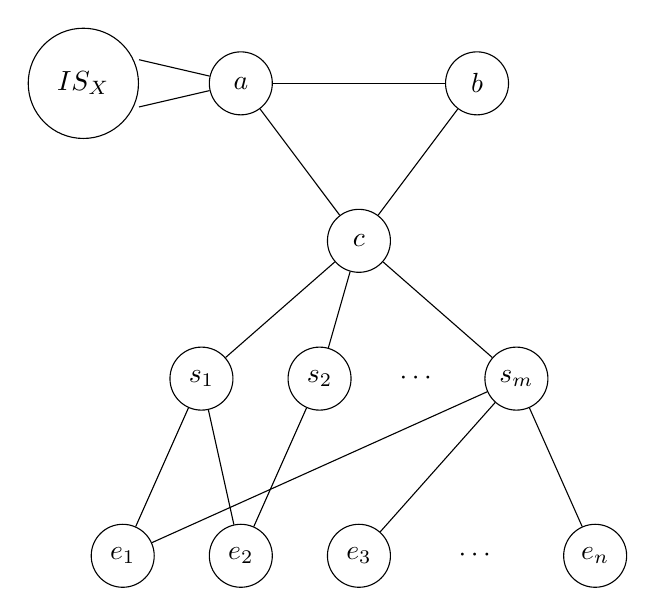
\begin{tikzpicture}[ 
        roundnode/.style={circle, draw=black, fill =white, minimum size=8mm},
        largenode/.style={circle, draw=black, minimum size=14mm},
        goldnode/.style={circle, draw=black, fill=red, minimum size=8mm}
        bluenode/.style={circle, draw=black, fill=red, minimum size=8mm},
    ]

    % Nodes
    \node[roundnode] (a) at (-1.5,3) {$a$};
    \node[roundnode] (b) at (1.5,3) {$b$};
    \node[roundnode] (c) at (0,1) {$c$};

    \node[largenode] (is) at (-3.5,3) {$IS_X$};

    \node[roundnode] (S1) at (-2,-0.75) {$s_1$};
    \node[roundnode] (S2) at (-.5,-0.75) {$s_2$};
    \node (dots) at (.75,-0.75) {$\cdots$};
    \node[roundnode] (Sm) at (2,-0.75) {$s_m$};

    \node[roundnode] (E1) at (-3,-3) {$e_1$};
    \node[roundnode] (E2) at (-1.5,-3) {$e_2$};
    \node[roundnode] (E3) at (0,-3) {$e_3$};
    \node (dotsE) at (1.5,-3) {$\cdots$};
    \node[roundnode] (En) at (3,-3) {$e_n$};

    % Edges
    \draw[-] (a) -- (b);
    \draw[-] (a) -- (c);
    \draw[-] (b) -- (c);

    \draw[-] (c) -- (S1);
    \draw[-] (c) -- (S2);
    \draw[-] (c) -- (Sm);

    \draw[-] (S1) -- (E1);
    \draw[-] (S1) -- (E2);
    \draw[-] (Sm) -- (E3);
    \draw[-] (S2) -- (E2);
    \draw[-] (Sm) -- (E1);
    \draw[-] (Sm) -- (En);

    \draw[-] (a) -- ($(is.east) + (0,0.3)$);

    % Second edge from 'a' to the east side of 'IS_X' slightly below center
    \draw[-] (a) -- ($(is.east) + (0,-0.3)$);
    \end{tikzpicture}
    \caption{Construction of a CRI instance with vertices $a,b$ from Set Cover.}
    \end{figure}\\\\
    \textbf{$k$-sized set cover $\Longrightarrow$ $\frac{\min(c_{G+T}(a),c_{G+T}(b))}{\max(c_{G+T}(a),c_{G+T}(b))}=1$.} For each set $S_i$ in the cover, construct the edge $bs_i$. Now every element vertex must be adjacent to a set vertex in the cover (by definition of a cover), and then each of these set vertices has a newly constructed edge to $b$. Thus each element vertex is distance 2 from $b$, and $k$ set vertices are distance 1 away from $b$. Now $c_{G+T}(b)=2(n+k)+1(2)+1(k)+2(m-k)+2(n)=4n+2m+k+2$. Similarly, $c_{G+T}(a)=1(n+k)+1(2)+2(m)+3(n)=4n+2m+k+2$. Then the ratio of $a$ and $b$'s closeness centrality must be 1, as desired.\\\\
    \textbf{No $k$-sized set cover $\Longrightarrow$ $\frac{\min(c_{G+T}(a),c_{G+T}(b))}{\max(c_{G+T}(a),c_{G+T}(b))}<1$.} As previously stated, in order to maximize the closeness ratio of $a$ and $b$, we decrease $b$'s closeness centrality as much as possible with $k$ edges.\\\\
    \begin{lemma}\ref{lem:set-incident}
        In this construction, if there is no $k$-sized set cover, there is always a set $T\subseteq V^2\backslash E$ of at most $k$ edges, all incident on both $b\in V$ and any set vertex, whose addition to the graph optimally improves the closeness centrality of $b$.
    \end{lemma}
    \begin{proof}
        Deferred to appendix.
    \end{proof}
    \noindent
    In other words, the set of edges which will optimally decrease $b$'s closeness centrality are all incident on $b$ and some set vertex. Therefore, the best $b$ can reduce its closeness centrality is by connecting itself to set vertices. This method can make $k$ set vertices distance 1 from $b$, and thus at most $n-1$ element vertices distance 2 from $b$, as there is no cover. 

    \begin{claim}
        In this construction, if there is no $k$-sized set cover, then there must exist some element vertex with no newly-added edge incident on it or any vertex of a set containing it.
    \end{claim}
    \begin{proof}
        Deferred to appendix.
    \end{proof}
    \noindent
    However, using the above claim, there must be some element which remains distance 3 from $b$. Then the closeness ratio of $a,b$ is:
    \[\frac{\min(c_{G+T}(a),c_{G+T}(b))}{\max(c_{G+T}(a),c_{G+T}(b))}<\frac{(n+k)+2+2m+3n}{2(n+k)+2+2m-k+2n+1}=\frac{4n+2m+k+2}{4n+2m+k+3}<1\]
\end{proof}
\noindent
We have shown that it is NP-hard to achieve a closeness centrality ratio of 1, but are smaller ratios achievable in polynomial time? By manipulating the size of the independent set connected to $a$ (for $\tau=1$, it was $n+k$ vertices) we can in fact prove a much stronger hardness result. 

\begin{theorem}
    Closeness Ratio Improvement is NP-Hard for $\tau\in(\frac{1}{2},1)$.
\end{theorem}
\noindent
We will go through the construction of a Closeness Ratio Improvement instance from Set Cover, but the analysis of yes and no cases is deferred to the appendix.
\begin{proof}
    Fix an arbitrary $\tau\in(\frac{1}{2},1)$. Consider an instance of Set Cover with $m$ sets, $n$ elements, and $k\in\mathbb{N}$ which satisfies $\frac{2m+4n+k}{1+2m+4n+k}\geq\tau^2$. This fraction converges to $1$ as we increase $m,n,k$, and $\tau^2<1$ when $\tau\in(\frac{1}{2},1)$, so we should always be able to find $m,n,k$ that satisfy this inequality. Use the same construction of $G$ described in the proof of Theorem  and depicted in Figure. However, now let $X$ (the number of vertices in the independent set attached to $a\in V$) be an integer in the interval $(\frac{2+2m+3n-\tau(2+2m-k+2n+1)}{2\tau-1},$\\$\frac{2+2m+3n-\tau(2+2m-k+2n)}{2\tau-1}]$. We know such an integer always exists by Lemma. \\\\
    We claim that there exists a $k$-sized set cover of $U$ if and only if there is a set $T$ of at most $k$ edges such that $\frac{\min(c_{G+T}(a),c_{G+T}(b))}{\max(c_{G+T}(a),c_{G+T}(b))}\geq\tau$.
\end{proof}



%%-------------------------------------------------------------------------------------------------
%% CUT STOP: preserve the command below to generate the reference list


\section{$\frac{1}{2}$-Approximation}
To restate the problem, we are given a graph $G$, vertices $a,b$ and an edge budget $k$. In the decision variant of this problem, we are given a target ratio of $\tau$, but generally we would like to make the ratio of $a$ and $b$'s closeness centrality in the augmented graph as close to 1 as possible. \\\\
Observe that if $a$ and $b$ are ever connected, the worst possible ratio is $\frac{1}{2}$. This happens when every vertex other than $a,b$ in the graph is directly connected to $b$, and $a$'s only neighbor is $b$ itself (see Figure). For large $n$, $b$'s closeness centrality is $1$ times $n$ vertices, while $a$'s is $2$ times $n$ vertices, giving us closeness ratio of $\frac{1}{2}$. If $a$ was closer than $b$ to any vertex, then the numerator would increase and denominator would decrease, giving us a better ratio. Similarly, if any vertex was further than distance 1 from $b$, we would get a better ratio (think $\frac{2}{3},\frac{3}{4}$, etc.). In short, with $a$ and $b$ connected, we guarantee a closeness ratio at least $\frac{1}{2}$.
\begin{figure}
    \centering
    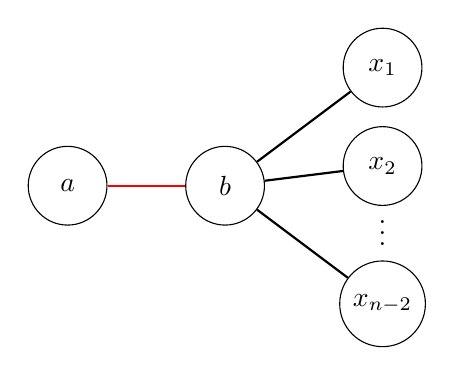
\begin{tikzpicture}[
        node/.style={circle, draw=black, minimum size=1cm},
        edge/.style={thick, -}
    ]
    
    % Define nodes
    \node[node] (A) at (0, 0) {$a$};
    \node[node] (B) at (2, 0) {$b$};
    
    % Draw edge between A and B
    \draw[edge, thick, red] (A) -- (B);
    
    % Define and connect nodes X_1 to X_n
    \node[node] (X1) at (4, 1.5) {$x_1$};
    \node[node] (X2) at (4, 0.25) {$x_2$};
    \node at (4, -0.5) {$\vdots$}; % Dots to represent continuation
    \node[node] (Xn) at (4, -1.5) {$x_{n-2}$};
    
    % Connect B to each X node
    \draw[edge] (B) -- (X1);
    \draw[edge] (B) -- (X2);
    \draw[edge] (B) -- (Xn);
    
    \end{tikzpicture}
    \caption{Worst case of closeness ratio when $a$ and $b$ are connected.}\label{2-apx}
\end{figure}\\\\
Now consider the algorithm, given $k\geq 1$ edges, which simply adds the edge $ab$ (if it does not already exist in the graph). As we just argued, our closeness ratio is now at least $\frac{1}{2}$ (though it might be better). This agrees very well with our hardness results, as we showed getting a target ratio greater than $\frac{1}{2}$ in all cases is NP-hard, but getting a target ratio of exactly $\frac{1}{2}$ is easy (in fact, it only requires one edge). \\\\
Furthermore, this strategy is a $\frac{1}{2}$-approximation for CRI. Whatever ratio an optimal efficient algorithm (which we do not know how to find, as this problem is NP-hard) would achieve on an instance of CRI, our algorithm will never get a ratio less than half of that value. This follows from the observation that, simply by our definition of closeness ratio, a ratio better than 1 is not possible. Thus is we guarantee a ratio of $\frac{1}{2}$, we guarantee that our algorithm produces no worse than $\frac{1}{2}$ of the optimal ratio. \\\\
An important distinction in this section is the difference between \textit{target} ratio and \textit{approximation} ratio. The approximation ratio is the ratio of the closeness ratio our algorithm achieves over the closeness ratio achieved by an optimal algorithm. Connecting $ab$ immediately achieves a target ratio of $\frac{1}{2}$, and as the best possible closeness ratio achievable is $1$, this strategy necessarily forms \textit{at least} at $\frac{1}{2}$ approximation. However, it is possible that this strategy is in fact better than a $\frac{1}{2}$-approximation. That is, all the problem instances where this strategy gets a ratio of $\frac{1}{2}$, an optimal strategy actually cannot get a ratio of 1 (meaning then the ratio of our ratio over optimal ratio is greater than $\frac{1}{2}$).\\\\
TIGHTNESS OF 1/2 EXAMPLE.
\section{Hardness of Approximation}
\begin{theorem}
    hardness of approximation.
\end{theorem}




\bibliographystyle{abbrvnat}
\bibliography{refs}


\newpage
\appendix
\section{Appendix Section}
\begin{claim} \label{clm:incident}
    Given a graph $G=(V,E)$, $v\in V$, $k\in\mathbb{N}$, and a set of edges $S\subseteq V^2\backslash E$ of size at most $k$ where at least one edge in $S$ is not incident on $v$, there must always exist a set $T\subseteq V^2\backslash E$ such that $|T|\leq|S|$ and $c_{G+T}(v)<c_{G+S}(v)$.
\end{claim}
\begin{proof}
    Define the edge in $S$ not incident on $v$ as $xy$, using its endpoints $x,y\in V$. Without loss of generality, suppose $d_{G+S}(v,x)\leq d_{G+S}(v,y)$. For any vertex $z\in V$, we have two cases: either the shortest path from $v$ to $z$ in $G+S$ uses the edge $xy$ or it does not. In either case, with the edge set $T=(S\backslash\{xy\})\cup\{vy\}$, we will show that $d_{G+T}(v,z)\leq d_{G+S}(v,z)$.\\\\
    If the path from $v$ to $z$ in $G+S$ uses the edge $xy$, then $d_{G+S}(v,z)$ can be expressed as $d_{G+S}(v,x)+1+d_{G+S}(y,z)$. Note that the assumption about the relative distances of $x,y$ to $v$ guarantees that the shortest path from $v$ to $z$ crosses over $xy$ instead of $yx$, as $d_{G+S}(v,x)\leq d_{G+S}(v,y)<d_{G+S}(v,y)+d_{G+S}(y,x)$. Then in $G+T$,
    \[d_{G+T}(v,z)=d_{G+T}(v,y)+d_{G+T}(y,z)=1+d_{G+S}(y,z)\]\[<d_{G+S}(v,x)+1+d_{G+S}(y,z)=d_{G+S}(v,z).\]
    If the path from $v$ to $z$ in $G+S$ does not use the edge $xy$, then removing it and replacing it with a new edge cannot make the distance between $v$ and $z$ any greater, it can only decrease it. Thus in either case, $d_{G+T}(v,z)\leq d_{G+S}(v,z)$. As this is true for every vertex $z\in V$, and this inequality is strict when $z=y$, $c_{G+T}(v)<c_{G+S}(v)$, as desired.
\end{proof}

\begin{lemma} \label{lem:incident}
    Given a graph $G=(V,E)$, $v\in V$ and $k\in\mathbb{N}$, there is always a set $T\subseteq V^2\backslash E$ of at most $k$ edges, all incident on $v$, whose addition to the graph optimally improves the closeness centrality of $v$.  
\end{lemma}
\begin{proof}
    Assume not. That is, suppose the set $S$ of $k$ edges which optimally improved the closeness centrality of $v$ were not all incident on $v$. This means at least one edge in $S$ is not incident on $v$, implying the existence of some set $T$ of size at most $k$ such that $c_{G+T}(v)<c_{G+S}(v)$ (by Claim~\ref{clm:incident}), contradicting the assumption that $S$ optimally improved the closeness centrality of $v$.
\end{proof}

\begin{claim} \label{clm:noedges}
    Given a graph of the construction provided in Figure~\ref{cri-reduction} derived from a set cover instance with $m$ sets, $n$ elements and $k\in\mathbb{N}$, if there is no $k$-sized set cover, then there must exist some element vertex with no newly-added edge incident on it or any vertex of a set containing it.
\end{claim}
\begin{proof}
   Assume not. That is, every element vertex \textit{does} have a new edge incident on it or one of the set vertices containing it. For any element vertex that is the endpoint of a new edge, simply reconstruct this edge to one of the set vertices adjacent to this element. Now we have identified $k$ edges incident only on set vertices such that every element is the neighbor of at least one such set vertex, and thus we have identified a $k$-sized set cover (a contradiction). 
\end{proof}

\begin{claim} \label{clm:set-incident}
    Given a graph of the construction provided in Figure~\ref{cri-reduction} derived from a set cover instance of $m$ sets, $n$ elements and $k\in\mathbb{N}$ with no $k$-sized set cover, given a set of at most $k$ edges $S\subseteq V^2\backslash E$, all incident on $b\in V$, if at least one edge is not incident on a set vertex, then there must exist a set $T\subseteq V^2\backslash E$ such that $|T|=|S|$ and $c_{G+T}(b)\leq c_{G+S}(b)$.
\end{claim}

\begin{proof}
    Suppose $S\subseteq V^2\backslash E$ is a set of $k$ edges which  contains only edges incident on $b$, but at least one edge is not incident on a set vertex. Given $b$ is connected to $a$ and $c$, this implies that there must exist an edge in $S$ which is connected a vertex $x_i$ in the independent set or an element vertex $e_i$. \\\\
    In the first case, this edge reduces the closeness centrality of $b$ by at most 1 --- it has changed $d(x_i,b)$ from 2 to 1, but not made $b$ closer to any other vertices. If we instead connect $b$ to a set vertex $s_i$, then $d(s_i,b)$ has been changed from 2 to 1, meaning this edge reduces the closeness centrality of $b$ by at least as much as the edge $b-x_i$. \\\\
    If the edge not incident on a set vertex instead connects $b$ to an element vertex $e_i$, this edge reduces the closeness centrality of $b$ by at most 2 --- it has changed $d(e_i,b)$ from 3 to 1, but not made $b$ closer to any other vertices. As there is no $k$-sized set cover, Claim~\ref{clm:noedges} tells us there must be some element vertex $e_j$ with no new edges incident on it or any set containing it. So instead connect $b$ to a set vertex $s_j$, where $e_j\in S_j$. then both $d(s_j,b)$ and $d(e_j,b)$ have been changed from 2 to 1, meaning $b-s_j$ reduces the closeness centrality of $b$ by at least as much as the edge $b-e_i$. \\\\ 
    If we define the set $T$ as the set $S$, but with the above case-dependent substitutions made, then we have that $|T|=|S|$ and $c_{G+T}(b)\leq c_{G+S}(b)$, as desired.
\end{proof}

\begin{lemma} \label{lem:set-incident}
    Given a graph of the construction provided in Figure~\ref{cri-reduction} derived from a set cover instance of $m$ sets, $n$ elements and $k\in\mathbb{N}$ with no $k$-sized set cover, there is always a set $T\subseteq V^2\backslash E$ of at most $k$ edges, all incident on both $b\in V$ and any set vertex, whose addition to the graph optimally improves the closeness centrality of $b$.
\end{lemma}

\begin{proof}
    From Lemma~\ref{lem:incident}, we know that there exists a set $T$ of $k$ edges which optimally improves the closeness centrality of $b$ such that all edges in $T$ are incident on $b$ itself. What remains to be shown is that there exists such a set of edges where they are all incident on $b$ \textit{and} some set vertex $s_i$.\\\\
    Assume not. That is, all the sets of edges which optimally improve $b$'s closeness centrality contain only edges incident on $b$, but at least one edge not incident on a set vertex. Now consider one such set of edges $S$. Claim~\ref{clm:incident} gives us a set $S'$ with $c_{G+S'}(b)\leq c_{G+S}(b)$. If $S'$ still contains an edge incident on $b$, but not a set vertex, we can reapply Claim~\ref{clm:incident} to get a new set that improves $b$'s closeness centrality just as well. In fact, we can keep applying this claim until we have a set of $k$ edges $T$ such that $|T|=|S|$ and $c_{G+T}(b)\leq c_{G+S}(b)$ and all edges in $T$ are incident on both $b$ and any set vertex. However, we assumed that all the sets of edges which optimally improve $b$'s closeness centrality contain only edges incident on $b$, but must have at least one edge not incident on a set vertex, a contradiction. 
\end{proof}

\begin{lemma}\label{lem:integer}
    For $m,n,k\in\mathbb{N}$ and $\tau\in\left(\frac{1}{2},1\right]$, there exists an\\ $X\in\left(\frac{2+2m+3n-\tau(2+2m-k+2n+1)}{2\tau-1},\frac{2+2m+3n-\tau(2+2m-k+2n)}{2\tau-1}\right]$ such that $X\in\mathbb{N}$.
\end{lemma}
\begin{proof}
    Taking the difference of the bounds of the interval\\ $\left(\frac{2+2m+3n-\tau(2+2m-k+2n+1)}{2\tau-1},\frac{2+2m+3n-\tau(2+2m-k+2n)}{2\tau-1}\right]$, we get that the length of the interval is $\frac{\tau}{2\tau-1}$, which is greater than or equal to $1$ for all $\tau\in\left(\frac{1}{2},1\right]$. Therefore, the length of our interval is bounded below by 1, and so there must exist some integer $X$ within this interval. Furthermore, as the numerator and denominator of the bounds of this interval are positive when $m,n,k\in\mathbb{N}$ and $\tau\in\left(\frac{1}{2},1\right]$, $X\in\mathbb{N}$ as desired.
\end{proof}


\begin{theorem} \label{t2-hard}
    Closeness Ratio Improvement is NP-Hard for $\tau\in(\frac{1}{2},1)$.
\end{theorem}
\begin{proof}
    (Concluding the argument started earlier, with construction given).\\\\
    \textbf{$k$-sized set cover $\Longrightarrow$ $\frac{\min(c_{G+T}(a),c_{G+T}(b))}{\max(c_{G+T}(a),c_{G+T}(b))}\geq\tau$.} If there is a set cover, follow the same protocol as in the proof of Theorem~\ref{t1-hard} (connect $b$ to the $k$ set vertices representing sets in the cover). In this case, $c_{G+T}(a)=X+2+2m+3n$ and $c_{G+T}(b)=2X+2+2m-k+2n$. \\\\
    We want to show that the ratio we achieve is greater than or equal to $\tau$, but we must still ensure that our ratio is less than or equal to 1, else we violate our min/max definition of closeness ratio. Note that this was not a conceren when $\tau=1$, because we showed our ratio when there was a set cover was $1$ exactly. So we consider the case where $c_{G+T}(b)\geq c_{G+T}(a)$ and the case where $c_{G+T}(b)<c_{G+T}(a)$, and show that in both cases the ratio of $\frac{\min(c_{G+T}(a),c_{G+T}(b))}{\max(c_{G+T}(a),c_{G+T}(b))}\geq\tau$.\\\\
    If $c_{G+T}(b)\geq c_{G+T}(a)$, then
    \[\frac{\min(c_{G+T}(a),c_{G+T}(b))}{\max(c_{G+T}(a),c_{G+T}(b))}=\frac{X+2+2m+3n}{2X+2+2m-k+2n}\]\[\geq\frac{(\frac{2+2m+3n-\tau(2+2m-k+2n)}{2\tau-1})+2+2m+3n}{2(\frac{2+2m+3n-\tau(2+2m-k+2n)}{2\tau-1})+2+2m-k+2n}\geq\tau\]
    Alternatively, if $c_{G+T}(b)<c_{G+T}(a)$, then
    \[\frac{\min(c_{G+T}(a),c_{G+T}(b))}{\max(c_{G+T}(a),c_{G+T}(b))}=\frac{2X+2+2m-k+2n}{X+2+2m+3n}\]\[>\frac{2(\frac{2+2m+3n-\tau(2+2m-k+2n+1)}{2\tau-1})+2+2m-k+2n}{(\frac{2+2m+3n-\tau(2+2m-k+2n+1)}{2\tau-1})+2+2m+3n}=\frac{(2-2\tau)+2m+4n+k}{\tau+2m\tau+4n\tau+k\tau}\]
    As $\tau\in(\frac{1}{2},1)$, $2-2\tau>0$, implying:
    \[\frac{(2-2\tau)+2m+4n+k}{\tau+2m\tau+4n\tau+k\tau}>\frac{2m+4n+k}{\tau+2m\tau+4n\tau+k\tau}=\frac{1}{\tau}(\frac{2m+4n+k}{1+2m+4n+k})\]
    We chose our Set Cover instance such that $\frac{2m+4n+k}{1+2m+4n+k}\geq\tau^2$. Thus we have that:
    \[\frac{1}{\tau}(\frac{2m+4n+k}{1+2m+4n+k})\geq\frac{1}{\tau}(\tau^2)=\tau\]
    Thus in either case, if there is a set cover of $U$, we can add $k$ edges to $G$ to get a closeness ratio greater than or equal to $\tau$.\\\\
    \textbf{No $k$-sized set cover $\Longrightarrow$ $\frac{\min(c_{G+T}(a),c_{G+T}(b))}{\max(c_{G+T}(a),c_{G+T}(b))}<\tau$.} If there is no $k$-sized set cover, we use the same analysis from the proof of Theorem~\ref{t1-hard} to argue that the best way $b$ can reduce its closeness centrality is by connecting itself to set vertices. Furthermore, this method makes $k$ set vertices distance 1 from $b$, and thus $n-1$ element vertices distance 2 from $b$, but (using Claim~\ref{clm:noedges}) there must be some element which remains distance 3 from $b$. Then the closeness ratio of $a,b$ is:
    \[\frac{\min(c_{G+T}(a),c_{G+T}(b))}{\max(c_{G+T}(a),c_{G+T}(b))}=\frac{X+2+2m+3n}{2X+2+2m-k+2n+1}\]\[<\frac{(\frac{2+2m+3n-\tau(2+2m-k+2n+1)}{2\tau-1})+2+2m+3n}{2(\frac{2+2m+3n-\tau(2+2m-k+2n+1)}{2\tau-1})+2+2m-k+2n+1}=\tau\]
\end{proof}

\end{document}
